\begin{figure}[H]
\centering

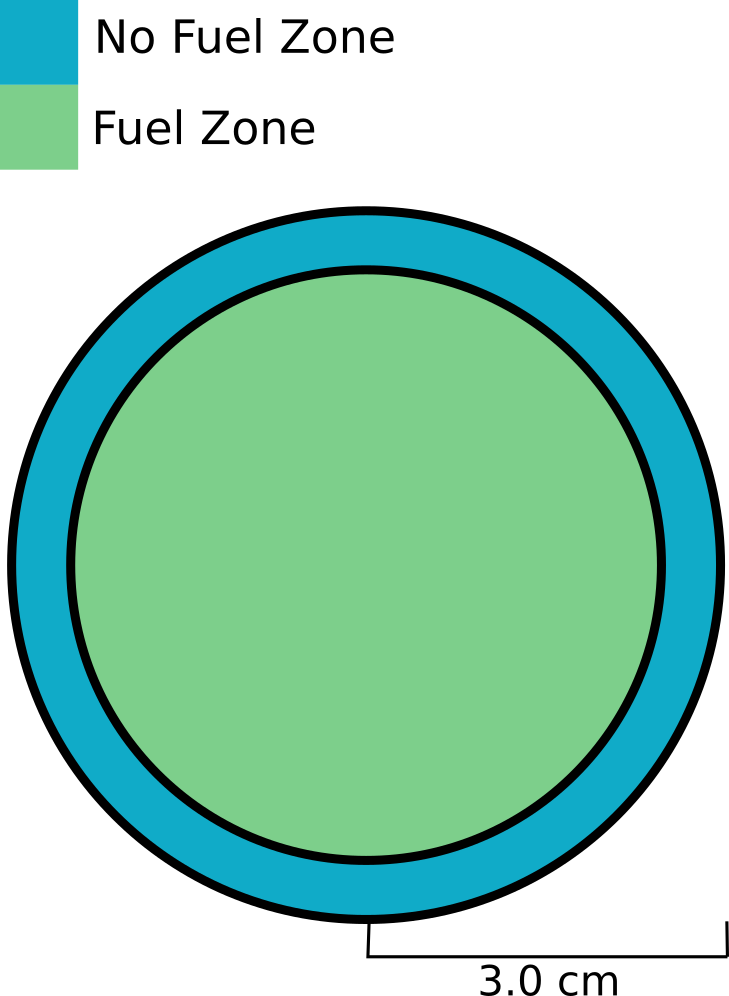
\includegraphics[width=0.5\linewidth]{figures/pebble-zones.png}
\caption{Pebble Zones}
\label{fig:pebb-zone1}
\end{figure}


\begin{table}[h!]
\centering

\caption{Pebble Parameters Used in Monte Carlo Simulations}
\begin{tabular}{ c  c }
\hline
Parameter & Value \\
\hline
Fueled-Center Radius [cm] & 2.5 \\
Graphite Outer Shell Thickness [cm] & 0.5 \\
Total Radius [cm] & 3.0 \\
TRISO Particles per Pebble & 18,000 \\
\hline
\end{tabular}
\label{table:peb-params}
\end{table}
